% !TEX root = ../../../Masterthesis.tex
\section{Hangar Management}
\begin{marginfigure}
\center
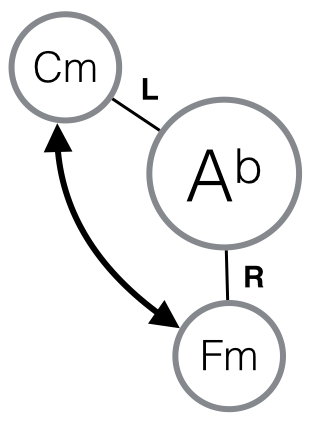
\includegraphics[width=0.6\linewidth]{ST_11_hangar_managment_1}
	\caption{ST 11: Hangar Management A}
	\label{ST_11_hangar_managment_1}
	%\setfloatalignment{b}
\end{marginfigure}
The scene begins after Kirk has been caught cheating on the ''Kobayashi Maru'' and he is now facing public reprimand. Admiral Barnett gets word that the Vulcan home-planet is under attack and he orders the cadets to report to Hanger One and await ship assignment. The scene shifts to the hanger where hundreds of people and shuttle crafts are preparing to leave. A variant on the new Giacchino Star Trek theme is heard in the french horns, accompanied by marching snare drums, staccato strings and tuned bass drums\footnote{The movie cue and the CD cue do differ; the movie features taikos to accent the beat whereas the CD track does not.}. The tonality is natural minor, \({iii}{\Leftrightarrow}{vi}\), centered around \aflat (figure \ref{ST_11_hangar_managment_1}). The Barracks Leader\footnote{Cameo by \textbf{Star Gate} fame ''Dr. Carson Beckett'': \textit{Paul McGillion}.} calls out the cadet assignments. When Kirk notices his name is not called, the music calms to a solo trumpet playing another variation of the new Star Trek theme--this time with a dorian feel. Kirk approaches the barracks leader and asks why his name was not called. The barracks leader informs Kirk that he is on academic suspension, meaning, he is grounded until the academy board's ruling. The music grinds to a halt while McCoy supports Kirk the best he can, but leaves to board the shuttle craft. The new Star Trek theme enters solemnly (figure \ref{ST_11_hangar_managment_2}) at m.12, signifying Kirk's standing, left behind and alone.

\begin{marginfigure}
\center
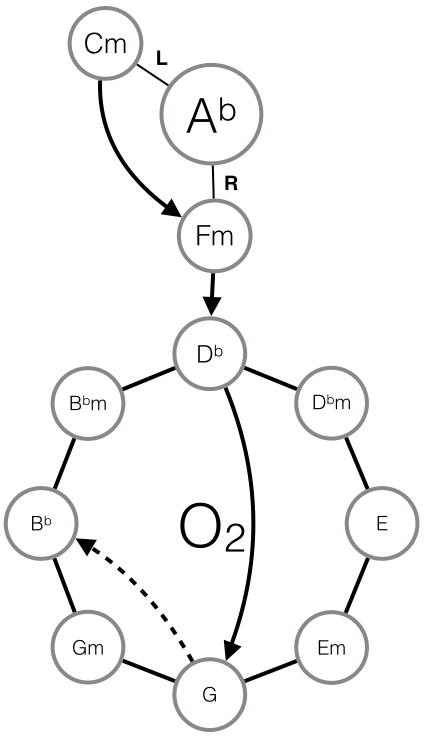
\includegraphics[width=\linewidth]{ST_11_hangar_managment_2}
	\caption{ST 11: Hangar Management B}
	\label{ST_11_hangar_managment_2}
	%\setfloatalignment{b}
\end{marginfigure}
 
\begin{marginfigure}
\center
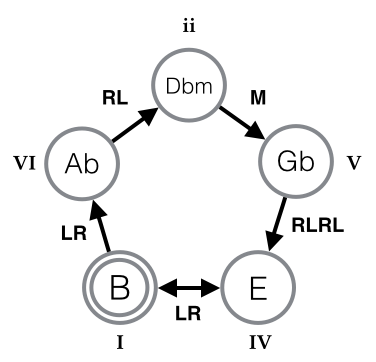
\includegraphics[width=\linewidth]{ST_11_hangar_managment_3}
	\caption{ST 11: Hangar Management D}
	\label{ST_11_hangar_managment_3}
	%\setfloatalignment{b}
\end{marginfigure}
McCoy has a change of mind, however, and the music makes a metric modulation while McCoy doubles back to fetch Kirk: ''Come with me!'' We now focus on Uhura who is assigned to the USS Farragut. Obviously displeased by this, she storms passed Kirk and McCoy who are discussing: ''Bones, where are we going?'', ''You'll see!'' A few strides later she meets Spock, her superior officer, asking why she was not picked out for the USS Enterprise. The music turns sweeter (figure \ref{ST_11_hangar_managment_3}), with the oboe playing a melody with a slight touch of something tongue-in-cheek, perhaps portraying the ferocious femininity emitting from Uhura as she makes an inarguable case for herself. Spock tries to defend his decision by placing Uhura on the USS Farragut on the basis of ''avoiding the appearance of favoritism.''. This does not go down well with Uhura who simply states: ''No. I'm assigned to the Enterprise.''. Spock swiftly and wisely makes an adjustment in the rosters to confirm.

''What are you doing?!'' Kirk asks. ''I'm doing you a favor.'' McCoy replies. The music is still calm, but the sonority has changed from dorian to lydian. This gives us the feeling that something wonderful and fantastic is going to happen. And indeed it does; McCoy injects Kirk with a vaccine for some aggressive disease causing Kirk to experience some severe allergic reactions. McCoy drags Kirk to a shuttle craft, and the musical figure modulates from \dflat to E, raising the energy levels (figure \ref{ST_11_hangar_managment_4}). But instead of a call-and-response, a trumpet now plays hints of the original Star Trek theme. McCoy then invokes protocol and rank to let Kirk join the shuttle craft. At the very end of the sequence, the original Star Trek theme is heard.

\begin{marginfigure}
\center
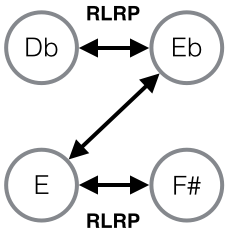
\includegraphics[width=0.7\linewidth]{ST_11_hangar_managment_4}
	\caption{ST 11: Hangar Management E}
	\label{ST_11_hangar_managment_4}
	%\setfloatalignment{b}
\end{marginfigure}

%-----------------------------------------------------------------------------
% PDF
%-----------------------------------------------------------------------------
\clearpage
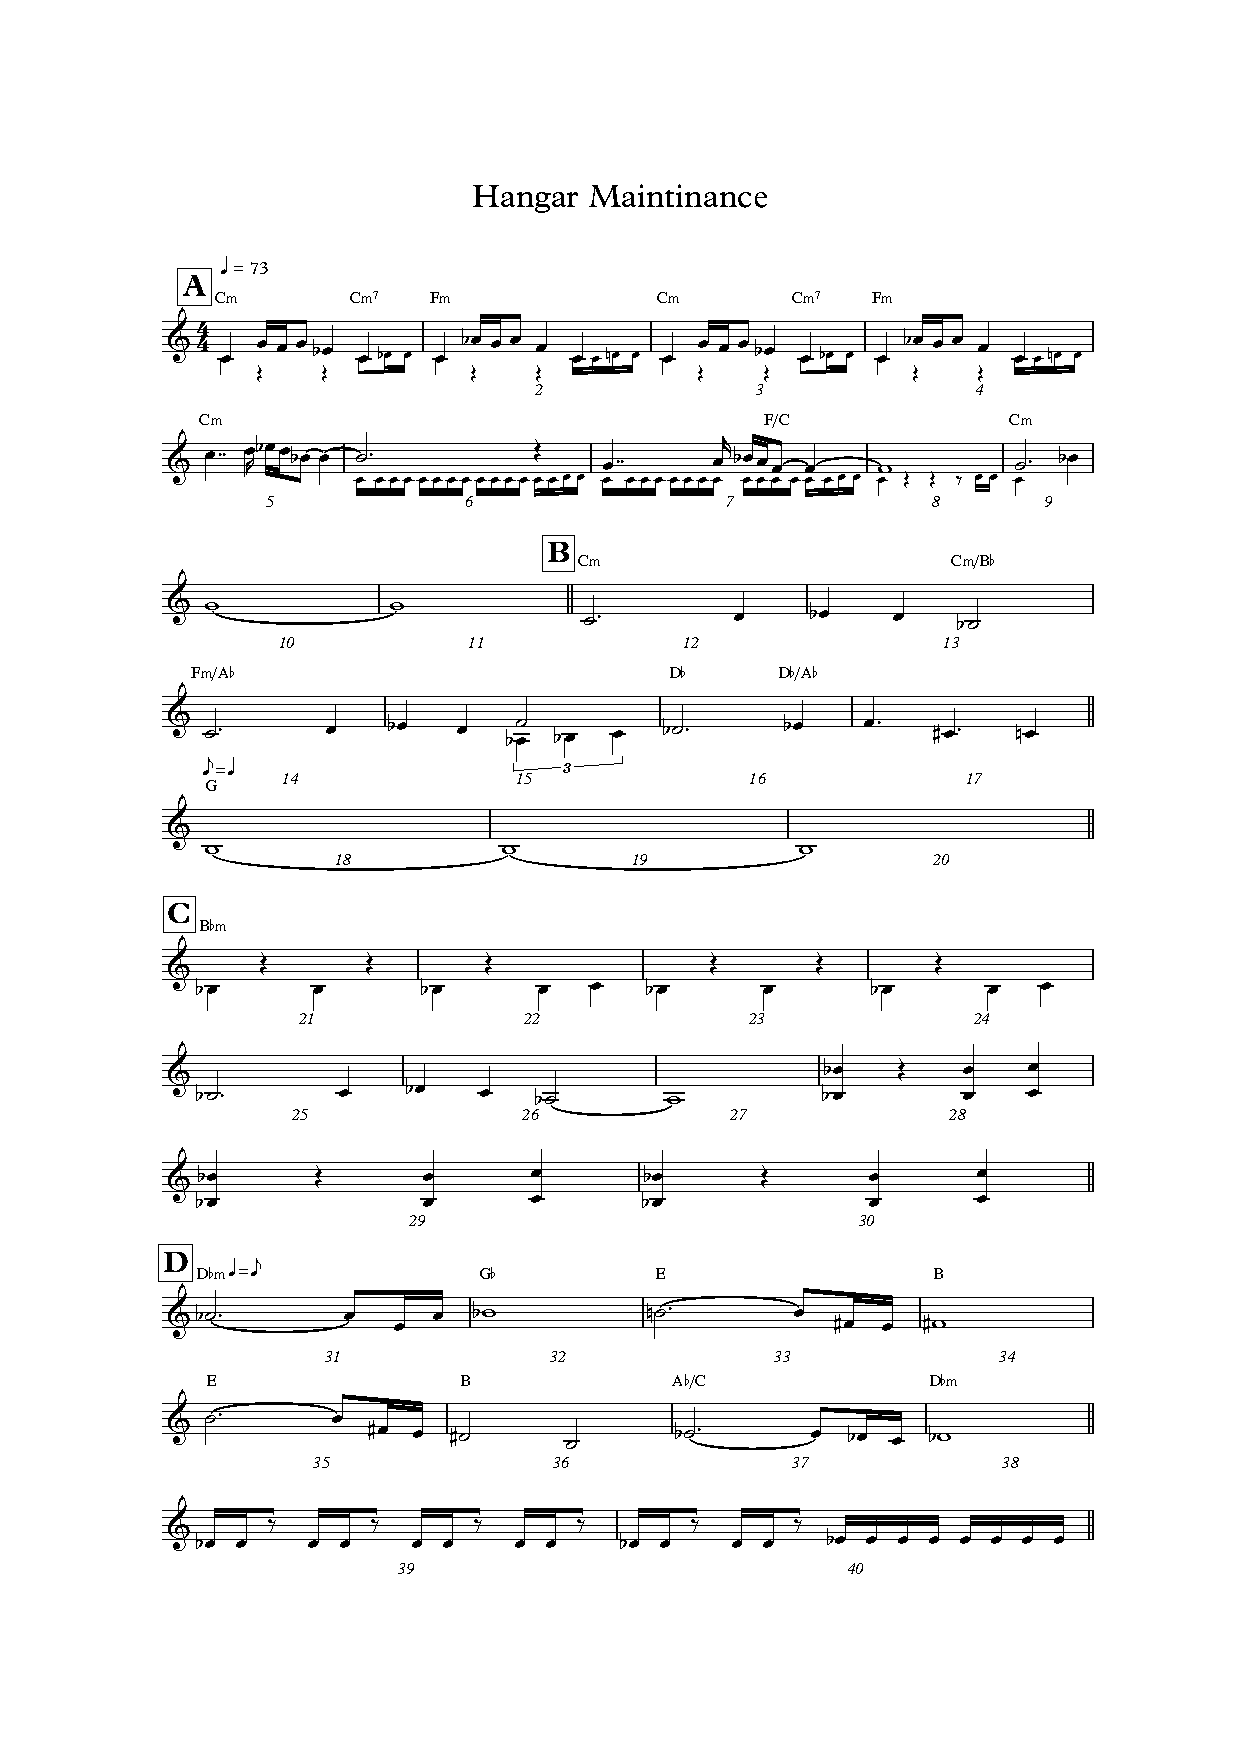
\includepdf[pages=-,pagecommand=\thispagestyle{fancy}]{pdf/st11/ST_11_13_hangar_management}

% Reviewed